% !TEX program = xelatex
\documentclass[aspectratio=1610,multi,rgb]{beamer}
%\documentclass[12pt]{article}
%\usepackage[noxcolor]{beamerarticle}

%\usetheme{Luebeck}
%\usetheme{Marburg}
%\usetheme{Goettingen}
%\usetheme{Hannover}
\usecolortheme{whale}

\usepackage[edges]{forest}
\usepackage{chronology}
\usepackage{ragged2e}
\let\raggedright=\RaggedRight
\usepackage[spanish]{babel}
\usepackage{multimedia}
\usepackage{pgfplots}
\usepackage{scrextend}
\usepackage{multicol}
\usepackage{geometry}
\usepackage{fontspec}
\usepackage{tabularx}
\usepackage{graphicx}
\usepackage{booktabs}
\usepackage{listings}
\usepackage{fancybox}
\usepackage{textpos}
\usepackage{xcolor}
\usepackage{subfig}
\usepackage{color}
\usepackage{calc}
\usepackage{tikz}
\usepackage{empheq}
\usepackage[T1]{fontenc}
\usepackage{lmodern}

\usepackage[backend=biber,
	    style=authoryear-icomp,
]{biblatex}
\addbibresource{bibliography.bib}

%\usepackage[square,numbers]{natbib}
%\bibliographystyle{abbrvnat}
%\setcitestyle{authoryear,open={(},close={)}} %Citation-related commands

\definecolor{lightgreen}{HTML}{90EE90}
\usetikzlibrary{arrows.meta,shadows.blur}
\colorlet{myyellow}{yellow!50}

\usefonttheme{professionalfonts} % using non standard fonts for beamer
\setmainfont{IBM Plex Sans}

\setbeamertemplate{navigation symbols}{}

\newcommand{\boxedeq}[2]{\begin{empheq}[box={\fboxsep=6pt\fbox}]{align}\label{#1}#2\end{empheq}}
\newcommand{\coloredeq}[2]{\begin{empheq}[box=\colorbox{lightgreen}]{align}\label{#1}#2\end{empheq}}

\newcommand{\fig}[3]{
\begin{columns}
\column{0.4\textwidth}
\begin{figure}[htp] \includegraphics[height=0.5\textheight,width=0.9\textwidth,
keepaspectratio]{#1}\caption{#2}\end{figure}
\column{0.6\textwidth}#3
\end{columns}
}

\newcommand{\titleframe}[1]{
\begin{frame} \null\hfill\huge{\shadowbox{#1}}\hspace{1cm} \end{frame}}

\newcommand{\ssec}{Título de subsección}

\newcommand{\tabitem}{~~\llap{\textbullet}~~}

\title{Ecuaciones de estado multiparamétricas - GERG 2008}
\author{Federico Benelli}
\institute{IPQA}
\date{28 de Junio 2021}


\begin{document}
\nocite{*}

\begin{frame}\maketitle\end{frame}

\section{Introducción}
\titleframe{Introducción}

\begin{frame}{Introducción}
	El conocimiento de propiedades termodinámicas de gases naturales y
	mezclas de sus compuestos es de indispensable importancia para la
	ingeniería básica de procesos técnicos.\\
	El procesado, transporte y almacenamiento de gases naturales requiere
	el cálculo de propiedades para un amplio espectro de composiciones y
	condiciones de operación.\\~\\
	Estas propiedades pueden ser calculadas mediante \textbf{Ecuaciones
	de estado}
\end{frame}

\subsection{Ecuaciones de estado}
\begin{frame}{Introducción}{Ecuaciones de estado (EOS)}
	$X(P,V,T,...)$
	\small{
	\begin{itemize}
	\item EOS Cúbicas
	\begin{itemize}
		\item Peng-Robinson
		\item Redlich-Kwong
		\item Soave-Redlich-Kwong
	\end{itemize}
	\item EOS Moleculares
	\begin{itemize}
		\item SAFT
	\end{itemize}
	\item EOS Multiparamétricas
	\begin{itemize}
	\item AGA8 
	\begin{equation}
	\label{eq_aga8}
	Z = 1 + \frac{\delta B}{K^3} - \delta  \sum\limits_{n=13}^{18} C_n^*
	T^{u_n}(b_n-c_nk_n\delta ^{k_n})\delta ^{b_n} \exp (-c_n \delta ^{k_n})
	\end{equation} 

	\item GERG
	\begin{equation}
	\label{eq_gerg}
	\alpha(\rho, \tau, \overline{x}) = 
		\alpha^o(\rho, T, \overline{x})
		+ \sum\limits_{i=1}^N x_i\alpha_{oi}^r(\delta,\tau)
		+ \Delta\alpha^r(\delta,\tau,\overline{x})
	\end{equation}
	\end{itemize}
	\end{itemize}
	}
\end{frame}


\subsection{Ecuaciones de estado multiparamétricas}
\subsubsection{Antecedentes}
\begin{frame}
	\frametitle{Ecuaciones de estado multiparamétricas}
	\framesubtitle{Antecedentes}
	\center{
	\begin{chronology}[5]{1980}{2020}{75ex}[\textwidth]
		\tiny{
		\event{1985}{Base de datos GERG}
		\event{1992}{Desarrollo AGA8}
		\event{1995}{Jaeschke - Cálculo de $c_p$ gas ideal}
		\event{1996}{Lemmon - Desarrollo de Departure Function}
		\event{2002}{\parbox{13em}{Span y Wagner \\ Ecuaciones compuestos puros}}
		\event{2004}{GERG 2004 - Ecuación de estado para mezclas}
		\event{2008}{\parbox{13em}{GERG 2008 \\ Agregado de 3 compuestos}}
	}
	\end{chronology}
	}
\end{frame}

\subsubsection{Estructura General}
\begin{frame}{Ecuaciones de estado multiparamétricas}{Estructura General}
	Son ecuaciones que se basan en el ajuste de datos experimentales
	para describir la energía libre de Helmholtz residual.

	\onslide<1>{
	\begin{block}{Estructura General}
	\begin{equation}
		\frac{A}{RT} = \alpha(\delta, \tau, \overline{x}) = 
		\alpha^o(\rho, T, \overline{x}) 
		+ \alpha^r(\delta, \tau, \overline{x})
	\end{equation}
	\end{block}
	}
%
%	\onslide<2-4>{
%	\center{
%	\begin{tabular}{rl}
%		$\delta = \rho/\rho_r(\overline{x})$ &
%		$\tau = T_r(\overline{x})/T$
%	\end{tabular}
%	}
%	}
%	\onslide<3-4>{
%	\begin{equation}
%	\alpha^o(\rho,T,\overline{x}) = 
%		\sum\limits_{i=1}^{N}x_i [\alpha^o_{oi}(\rho, T) +
%		\ln(x_i)]
%	\end{equation}
%	}
%	\onslide<4>{
%	\begin{equation}
%	\alpha^r(\delta,T,\overline{x}) = 
%		\sum\limits_{i=1}^{N}x_i\alpha_{oi}^r(\delta, \tau)
%		+ \Delta\alpha^r(\delta,\tau,\overline{x})
%	\end{equation}
%	}

\end{frame}

\section{GERG 2008}
\titleframe{GERG 2008}

\subsection{Origen}
\begin{frame}{Ecuación GERG}{Origen}
	Ecuación \emph{AGA8-DC92} (\ref{eq_aga8}) limitada a rangos acotados
	($250K \le T \le 350 K$ y $p < 30 MPa$).  Además, presenta mayores
	incertidumbres al tratar con mezclas inusuales.
	\begin{block}{Objetivos GERG}
	\begin{itemize}
	\item Válida en toda la región de fluidos.
	\item Incertidumbres $\le$ a 0,1\% en $\rho$ y $w$.
	\item Incertidumbres $\le$ a 1\% en otras propiedades.
	\item Aceptable en rangos con datos de baja calidad.
	\item Estructura simple.
	\end{itemize}
	\end{block}
\end{frame}

\subsection{Estructura}
\begin{frame}[t]{Ecuación GERG 2008}{Estructura}
	{\fontsize{8pt}{8pt}\selectfont
	\begin{forest}
	for tree={
	fit=band,
	grow'=0,
	parent anchor=children,
	child anchor=parent,
	anchor=parent,
	if n children=0{folder}{},
	edge path'={(!u.parent anchor) -- ++(5pt,0) |- (.child anchor)},
	},
	where n=1{
	calign with current edge
	}{},
	[GERG 2008, tier=l0, 
		[Término Ideal, tier=l1
			[\parbox{12em}{
				$n^o_{oi,1-7}$,
				$\vartheta^o_{oi,4-7}$
			},
			tier=l3]
		]
		[Término Residual, tier=l1
			[Sustancias Puras, tier=l2
				[
				\parbox{12em}{
				$n_{oi,1-K_e}$,
				$d_{oi,1-K_e}$,\\
				$t_{oi,1-K_e}$},
				tier=l3]
				[$c_{oi,K_p-K_e}$,tier=l3]
			]
			[Departure Function, tier=l2
				[$n_{ij,1-K_e}$
				$d_{ij,1-K_e}$
				$t_{ij,1-K_e}$,tier=l3]
				[
				\parbox{12em}{$\eta_{ij,K_p-K_e}$,
				$\varepsilon_{ij,K_p-K_e}$ \\
				$\beta_{ij,K_p-K_e}$,
				$\gamma_{ij,K_p-K_e}$}
				,tier=l3]
			]
		]
		[Funciones Reductoras, tier=l1
			[$1/\rho_r(\overline{x})$, tier=l2
				[$\beta_{\nu,N}$,tier=l3]
				[$\gamma_{\nu,N}$,tier=l3]
			]
			[$T_r(\overline{x})$, tier=l2
				[$\beta_{T,N}$,tier=l3]
				[$\gamma_{T,N}$,tier=l3]
			]
			]
	]
	\end{forest}
	}

	\begin{equation}
	\tag{\ref{eq_gerg}}
	\alpha(\rho, \tau, \overline{x}) = 
		\alpha^o(\rho, T, \overline{x})
		+ \sum\limits_{i=1}^N x_i\alpha_{oi}^r(\delta,\tau)
		+ \Delta\alpha^r(\delta,\tau,\overline{x})
	\end{equation}
\end{frame}

\subsubsection{Funciones reductoras}

\begin{frame}
	\frametitle{Funciones Reductoras}
	\framesubtitle{$\rho(\overline{x}), \tau(\overline{x})$}
	Son utilizadas para determinar las variables reducidas de mezclas.
	Se obtienen ajustando parámetros a datos de mezclas.
	\begin{columns}
	\column{0.6\textwidth}
	\small{
	\begin{block}{Condiciones}
		\begin{itemize}
		\item $x_i {\rightarrow 0}$ debe conectar suavemente
		a los parámetros de la sustancia pura.
		\item Describir tanto mezclas binarias como 
		multicomponentes.
		\item Su forma matemática no debe depender del orden
		de los componentes.
		\item Flexible como para describir formas simétricas
		y asimétricas  en mezclas equimolares.
		\item Deben asegurar valores físicamente razonables
		al usarse en las propiedades derivadas.
		\end{itemize}
	\end{block}
	}
	\column{0.5\textwidth}
		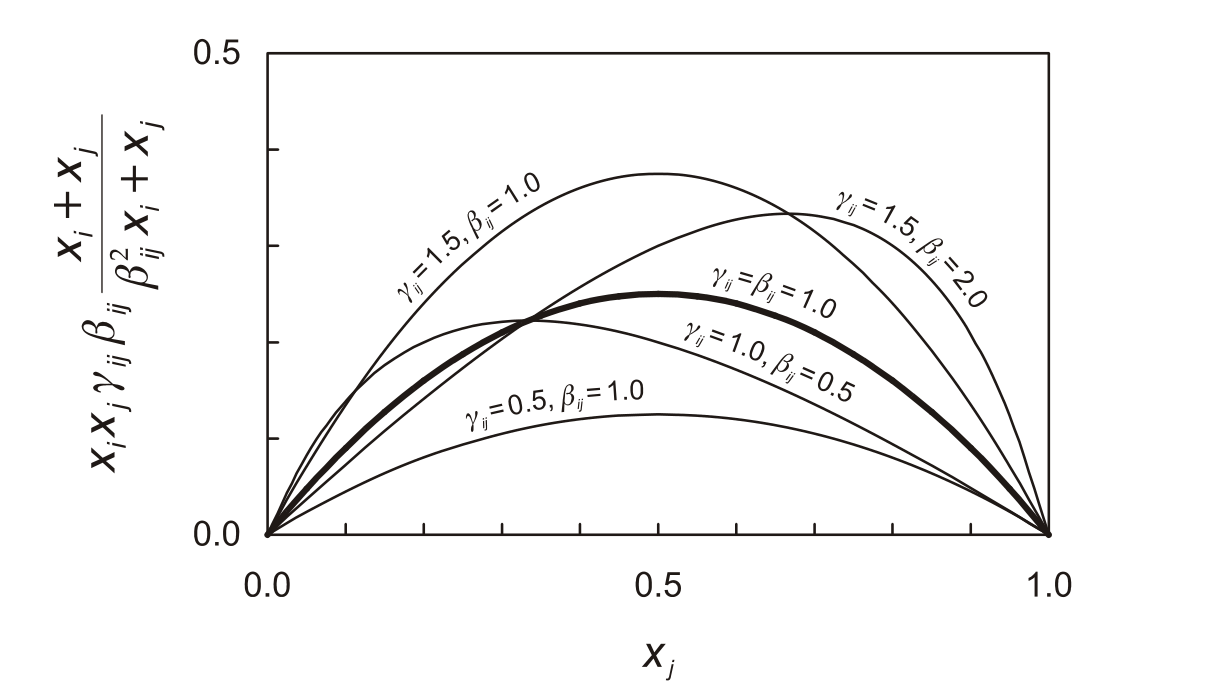
\includegraphics[width=\textwidth]{figs/equimolar_mix.png}
	\end{columns}
\end{frame}

\begin{frame}
	\frametitle{Funciones Reductoras}
	\framesubtitle{}
	Las funciones reductoras se utilizan para posteriormente obtener
	la densidad reducida $\delta$ y la temperatura reducida $\tau$. \\
	GERG-2008 utiliza funciones basadas en reglas de mezclado
	cuadráticas.
	\begin{equation}
	\frac{1}{\rho_r(\overline{x})} = 
		\sum\limits_{i=1}^{N}\sum\limits_{j=1}^{N}
		x_ix_j\beta_{\nu,ij}\gamma_{\nu,ij}
		\frac{x_i+x_j}{\beta_{\nu,ij}^2x_i+x_j}
		\frac{1}{8}\left(
			\frac{1}{\rho_{c,i}^{1/3}} +
			\frac{1}{\rho_{c,j}^{1/3}} +
		\right)^3
	\end{equation}
	\\~\\
	\begin{equation}
		T_r(\overline{x}) = 
		\sum\limits_{i=1}^{N}\sum\limits_{j=1}^{N}
		x_ix_j\beta_{T,ij}\gamma_{T,ij}
		\frac{x_i+x_j}{\beta_{T,ij}^2x_i+x_j}
		\left(
			T_{c,i} \cdot T_{c,j}
		\right)^{0.5}
	\end{equation}

	En casos donde no haya datos de calidad, los parámetros de ajuste 
	se ajustan a 1, convirtiendo la ecuación a una regla de mezclado 
	clásica.

\end{frame}

\subsubsection{Sustancia pura}
\begin{frame}{Término ideal}{$\alpha^0(\rho,T,\overline{x})$ -
	Término ideal}
	\begin{equation}
		\alpha^o(\rho,T,\overline{x}) = 
			\sum\limits_{i=1}^Nx_i[
				\alpha^o_{oi}(\rho,T) + \ln x_i
				]
	\end{equation}
	\begin{description}
	\item[\textbf{$x_i$}] Fracción molar compuesto $i$.
	\item[\textbf{$\alpha^o_{oi}(\rho,T)$}]
		Energía de Helmholtz compuesto 
		puro.
	\item[\textbf{$\ln x_i$}] Entropía de mezclado.
	\end{description}
\end{frame}

\begin{frame}
	\frametitle{Término ideal}
	\framesubtitle{$\alpha_{oi}^o(\rho,T)$ - Sustancia Pura}
	$\alpha_{oi}^o(\rho,T)$ corresponde a la energía libre de Helmholtz de
	la sustancia pura.
	Se obtiene a partir de la definición de la energía libre de Helmholtz:
	\begin{equation}
	a^o(\rho,T) = h^o(T)- RT - Ts^o(\rho,T)
	\end{equation}
	Que en el caso de un gas ideal se resuelve como:
	\begin{equation}
	a^o(\rho,T) = \left[\int_{{T_0}}^{{T}} {c_p^o} \: d{T} +h_0^o\right]
	 -RT - T \left[
		 \int_{{T_0}}^{{T}} {\frac{c_p^o-R}{T} } \: d{T} 
		 - R \ln \left(\frac{\rho}{\rho_o^o}\right) + s_0^o
		\right]
	\end{equation}

\end{frame}

\begin{frame}[t]
	\frametitle{Término ideal}
	\framesubtitle{$\alpha_{oi}^o(\rho,T)$ - Sustancia Pura}
	\cite{jaeschke_92} determinaron coeficientes para
	el cálculo de $c_p$. Con la aplicación de estos coeficientes en la
	integración anterior se obtiene:
	\\~\\	
	\begin{equation}
	\begin{aligned}
	\alpha_{oi}^o(\rho,T) =
		&  \ln \left(\frac{\rho}{\rho_{c,i}}\right) +
		\frac{R^*}{R} \left[n_{oi,1}^o + n_{oi,2} \frac{T_{c,i}}{T} +
		n_{oi,3}^o \ln\frac{T_{c,i}}{T}\right] \\~\\
		& + \sum\limits_{k=4,6} n_{oi,k}^o \ln
		\left(\left| \sinh
		\left(\vartheta_{oi,k}^o
			\frac{T_{c,i}}{T}
		\right) \right| \right)\\~\\
		& - \sum\limits_{k=5,7} n_{oi,k}^o \ln
		\left( \cosh
		\left(\vartheta_{oi,k}^o
			\frac{T_{c,i}}{T}
		\right) \right)\\
	\end{aligned}
	\end{equation}
\end{frame}


\subsubsection{Término residual}

\begin{frame}{Término residual}
	{$\sum\limits_{i=1}^N x_i\alpha_{oi}^r(\delta,\tau)
		+ \Delta\alpha^r(\delta,\tau,\overline{x})$}
		\begin{tabular}{p{0.6\textwidth}p{0.2\textwidth}<{\centering}}
	\tabitem El primer término corresponde a la combinación
		lineal de los compuesots puros.
	&
	$\sum\limits_{i=1}^N x_i\alpha_{oi}^r(\delta,\tau)$
	\\
	\tabitem El segundo término corresponde a una función denominada
	\emph{``Departure Function''}
	&
	$\Delta\alpha^r(\delta,\tau,\overline{x})$ \\
	\end{tabular}
\end{frame}



\begin{frame}
	\frametitle{Término residual}
	\framesubtitle{$\alpha_{oi}^r(\delta,\tau)$ - Forma funcional}
	Para poder realizar el ajuste de datos experimentales, es necesario
	establecer una estructura matemática que describa a la energía residual
	$\alpha_{oi}^r(\delta,\tau)$. 

	Se planteó una forma funcional como una combinación de sumatorias de
	dos tipos de términos:

	\begin{description}
	\onslide<1->{
	\item[Términos polinómicos]
	\begin{equation}
		\alpha_i^r = n_i\delta^{d_i}\tau^{t_i}
	\end{equation}
	\item[Términos Exponenciales]
	\begin{equation}
		\alpha_i^r = n_i\delta^{d_i}\tau^{t_i}e^{-\delta^{c_i}}
	\end{equation}}
	\onslide<2>{
	\item[Forma funcional]
	\begin{equation}
		\alpha^r(\delta,\tau) = 
		\sum\limits_{k=1}^{K_{Pol}}
		 n_k\delta^{d_k}\tau^{t_k}
		 + \sum\limits_{k=K_{Pol}+1}^{K_{Pol}+K_{Exp}}
		 n_k\delta^{d_k}\tau^{t_k}e^{-\delta^{c_k}}
	 \end{equation}}
	\end{description}
\end{frame}


\begin{frame}
	\frametitle{Término residual}
	\framesubtitle{	$\Delta\alpha^r(\delta,\tau,\overline{x})$
	- Departure Function}
	$\Delta\alpha^r(\delta,\tau,\overline{x})$ fue utilizada por primera
	vez por \cite{tillner_93} y \cite{lemmon_96} con el propósito de
	mejorar la precisión de modelos multi-fluidos. 
\end{frame}
\begin{frame}
	\frametitle{Término residual}
	\framesubtitle{	$\Delta\alpha^r(\delta,\tau,\overline{x})$
	- Departure Function}
	\onslide<1->{
	Originalmente se utilizaban en mezclas binarias:
	\begin{equation}
		\Delta\alpha^r(\delta,\tau,\overline{x}) =
		f^\Delta(x_1,x_2) \cdot \alpha_{12}^r(\rho,\tau)
	\end{equation}}
	\onslide<2->{
	Forma Generalizada:
	\begin{equation}
		\Delta\alpha^r(\delta,\tau,\overline{x}) =
		\sum\limits_{i=1}^{N-1}\sum\limits_{j=i+1}^{N}
		x_ix_jF_{ij}\alpha_{ij}^r(\delta,\tau)
	\end{equation}
	}
	\onslide<3->{
	Forma funcional de $\alpha_{ij}^r$:
	\begin{equation}
	\begin{aligned}
	\alpha_{ij}^r = & \sum\limits_{k=1}^{K_{Pol,ij}} 
		n_{ij,k} \delta^{d_{ij,k}} \tau^{t_{ij,k}}
		+\sum\limits_{k=K_{Pol,ij}+1}^{K_{Pol,ij} + K_{exp,ij}}
		n_{ij,k}\delta^{d_{ij,k}}\tau^{t_{ij,k}} \\
		& \exp
		\left[
		-\eta_{ij,k}
		\left(
			\delta - \varepsilon_{ij,k}
		\right)^2 
		- \beta_{ij,k}	\left(
			\delta - \gamma_{ij,k} 
		\right)
		\right] \\
	\end{aligned}
	\end{equation}
	}
\end{frame}

\subsection{Ajuste a datos experimentales}
\begin{frame}
	\frametitle{Ajuste de datos experimentales}
	\framesubtitle{}
	Tanto la energía de Helmholtz residual ($\alpha^r$) como la función de
	salida ($\Delta\alpha^r$) requieren un proceso de ajuste de parámetros:
	\begin{block}{}
	\begin{enumerate}
		\item Selección de datos.
		\item Ponderación de datos.
		\item Precorrelación de cantidades auxiliares.
		\item Ajuste linear según mínimos cuadrados.
		\item Ajuste no-linear.
	\end{enumerate}
	\end{block}
\end{frame}

\subsubsection{Base de datos}
\begin{frame}
	\frametitle{Ajuste a datos experimentales}
	\framesubtitle{Base de datos}

	Desde antes de 1985, el grupo GERG expande continuamente su base
	de datos relacionada a propiedades de mezclas y compuestos puros.\\~\\

	\begin{forest}
		[Base datos GERG
		[125000 Puntos experimentales
		[Mezclas binarias]
		[Gases naturales]
		[Mezclas multicomponente]]
		[650 Fuentes]]
	\end{forest}

\end{frame}

\begin{frame}
	\frametitle{Base de datos}
	\framesubtitle{Rangos de datos}
	La base de datos utilizada por GERG cubre tanto regiones de gas
	homogéneo, líquido y supercrítico como también estados de equilibrio
	líquido-vapor en rangos de $ 16 < T < 2500$ K y $P < 2000$ MPa.
	
	\begin{block}{Tipos de datos}
	\begin{itemize}
		\item $p \rho T$
		\item Capacidad calorífica isocórica $c_v$
		\item Velocidad del sonido: $w$
		\item Capacidad calorífica isobárica: $c_p$
		\item Diferencias de entalpía: $\Delta h$
		\item Densidad de líquido saturado: $\rho^{'}$
		\item VLE: $pTxy$
	\end{itemize}
	\end{block}
\end{frame}
\begin{frame}
	\frametitle{Base de datos}
	\framesubtitle{Tipos de datos}
	Estos datos se distribuyen como:

	\begin{itemize}
		\item 70\% $p \rho T$.
		\item 21\% Puntos VLE.
		\item 9\%  Otras propiedades.
	\end{itemize} 
	\begin{tikzpicture}
	\begin{axis}[
		height=5cm, width=10cm,
		symbolic y coords={$p \rho T$,VLE,Otros},
		ytick=data
	]
	\addplot[xbar,fill=blue] coordinates {
		(70,$p \rho T$)
		(21,VLE)
		(9,Otros)
	};
	\end{axis}
	\end{tikzpicture}

	
\end{frame}


\begin{frame}
	\frametitle{Base de datos}
	\framesubtitle{Incertidumbres de mediciones}
	\center{
	\begin{tabular}{rcc}
		\toprule
		Tipo de dato & Propiedad & Incertidumbre relativa (\%)    \\
		\midrule
		$p \rho T$ & $\Delta \rho/\rho$ 	  & (0,03 a 0,1)  \\
		$c_v$ 	   & $\Delta c_v/c_v$ 		  & (1 a 2) 	  \\
		$w$	   & $\Delta w/w$		  & (0,02 a 0,01) \\
		$c_p$	   & $\Delta c_p/c_p$		  & (1 a 2) 	  \\
		$\Delta h$ & $\Delta(\Delta h)/ \Delta h$ & (0,2 a 0,5)   \\
		$\rho^{'}$ & $\Delta \rho^{'}/\rho^{'}$   & (0,1 a 0,3)   \\
		VLE	   & $\Delta p_s/p_s$		  & (1 a 3)       \\
		\hline
		\hline
	\end{tabular}}
\end{frame}

\subsubsection{Métodos de ajuste}
\begin{frame}[t]
	\frametitle{Métodos de ajuste}
	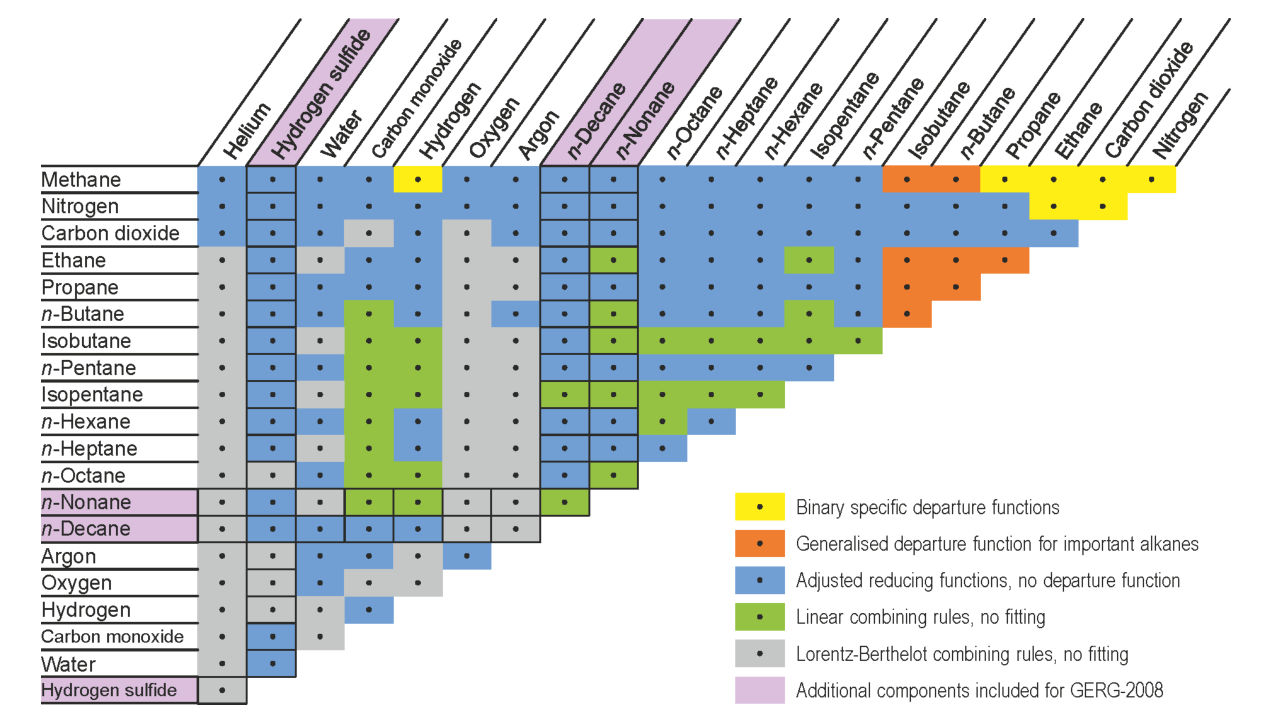
\includegraphics[width=\textwidth]{figs/compuestos.png}
\end{frame}
\begin{frame}
	\frametitle{Métodos de ajuste}
	\framesubtitle{Cálculo de propiedades medibles}
	La energía libre de Helmholtz no es medible, pero si se pueden obtener
	variables medibles a través de sus derivadas:
	\begin{equation}
		\frac{p(\delta,\tau,\overline{x})}{\rho RT} = 1 + \delta \alpha^r_{\delta}
	\end{equation} \\
	\begin{equation}
		\frac{w^2(\delta,\tau,\overline{x})}{RT}M = 
		1 + 2\delta \alpha_{\delta}^r + \delta^2\alpha_{\delta\delta}^r
		- \frac{(1+\delta \alpha^r_{\delta}- \delta \tau
		\alpha^r_{\delta\tau})^2}{\tau^2(\alpha_{\tau \tau}^o +
	\alpha^r_{\tau \tau})}
	\end{equation} \\
	\begin{equation}
		\frac{c_v(\delta,\tau,\overline{x})}{R} =
		-\tau^2(\alpha_{\tau\tau}^o + \alpha_{\tau\tau}^r)
	\end{equation} \\ 
	\begin{equation}
		Z(\delta, \tau, \overline{x}) = 1 + \delta\alpha^r_\delta
	\end{equation} \\
\end{frame}

\begin{frame}
	\frametitle{Métodos de ajuste}
	\framesubtitle{Cálculo de propiedades medibles}
	\textbf{Cálculo de VLE}
	\begin{equation}
		\varphi_i^{'}/\varphi_i^{''} = x_i^{''}/x_i^{'}
	\end{equation} \\
	\begin{equation}
		K_i = x_i^{''}/x_i^{'}
	\end{equation} \\
	\begin{equation}
		f_i = x_i\rho RT \exp \left(
			\frac{\partial n \alpha^r}{
		\partial n_i}\right)_{T,V,n_j} 
	\end{equation} \\
	\begin{equation}
		\ln \varphi_i = \left(
			\frac{\partial n \alpha^r}{
		\partial n_i}\right)_{T,V,n_j}  - \ln Z
	\end{equation} \\
	\begin{equation}
		x_i = (1-\beta)x_i^{'} + \beta x_i^{''}
	\end{equation}
\end{frame}

\section{Comparación de incertidumbres}

\titleframe{Comparación de incertidumbres}

\begin{frame}
	\frametitle{Comparación de incertidumbres}
	Se compararon datos experimentales con datos calculados con la
	ecuación GERG y otras ecuaciones de estado.
\end{frame}

\subsubsection{Densidad}
\begin{frame}
	\frametitle{Densidad}
	Densidad calculada en gases naturales.
	\center{
	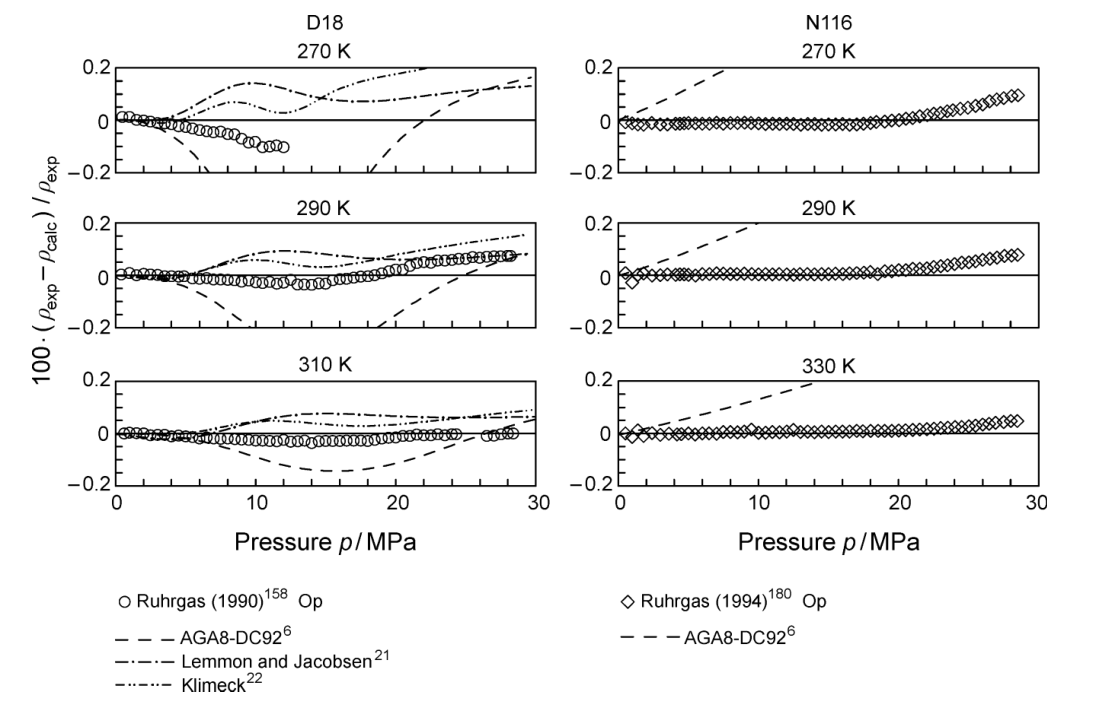
\includegraphics[width=0.9\textwidth]{figs/rho.png} 
	}
\end{frame}
\begin{frame}
	\frametitle{Densidad}
	Densidad calculada en gases naturales.
	\center{
	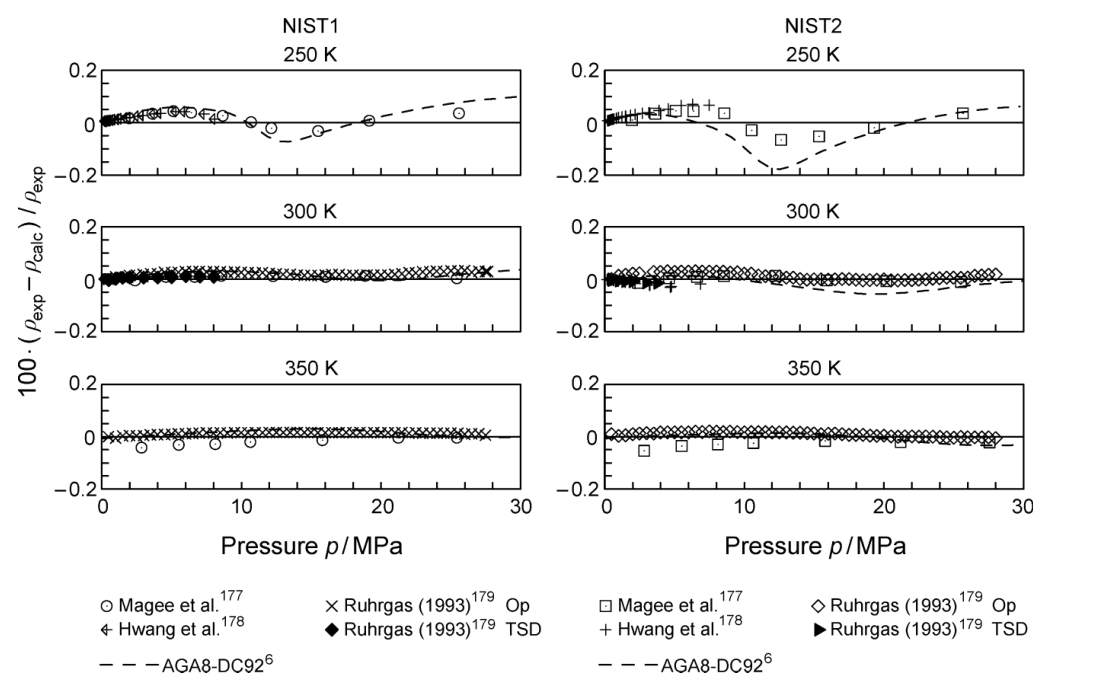
\includegraphics[width=0.9\textwidth]{figs/rho2.png} 
	}
\end{frame}

\subsubsection{Velocidad del sonido}
\begin{frame}
	Velocidad del sonido en mezcla Metano-Nitrógeno.
	\frametitle{Velocidad del sonido}
	\center{
	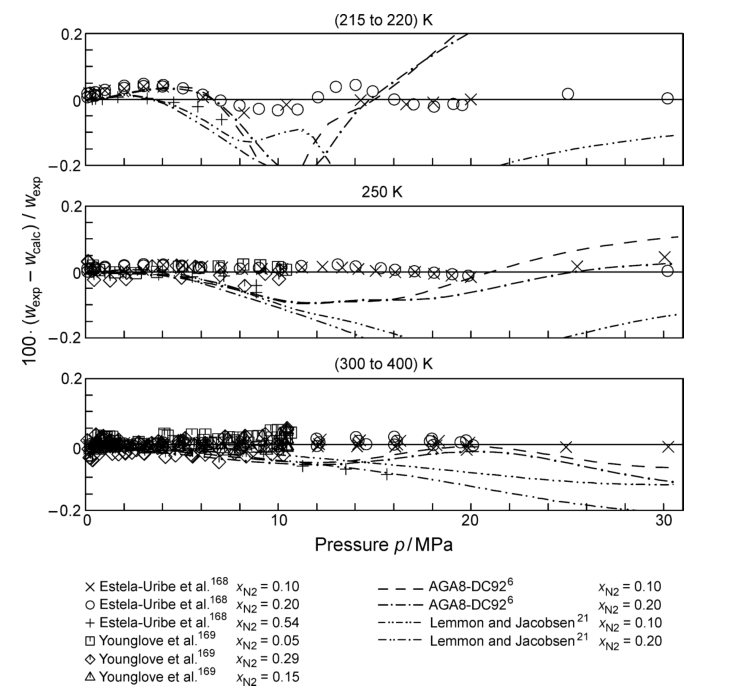
\includegraphics[width=0.65\textwidth]{figs/w.png} 
	}
\end{frame}

\begin{frame}[t]
	\frametitle{Velocidad del sonido}
	Velocidad del sonido en gases naturales.
	\center{
	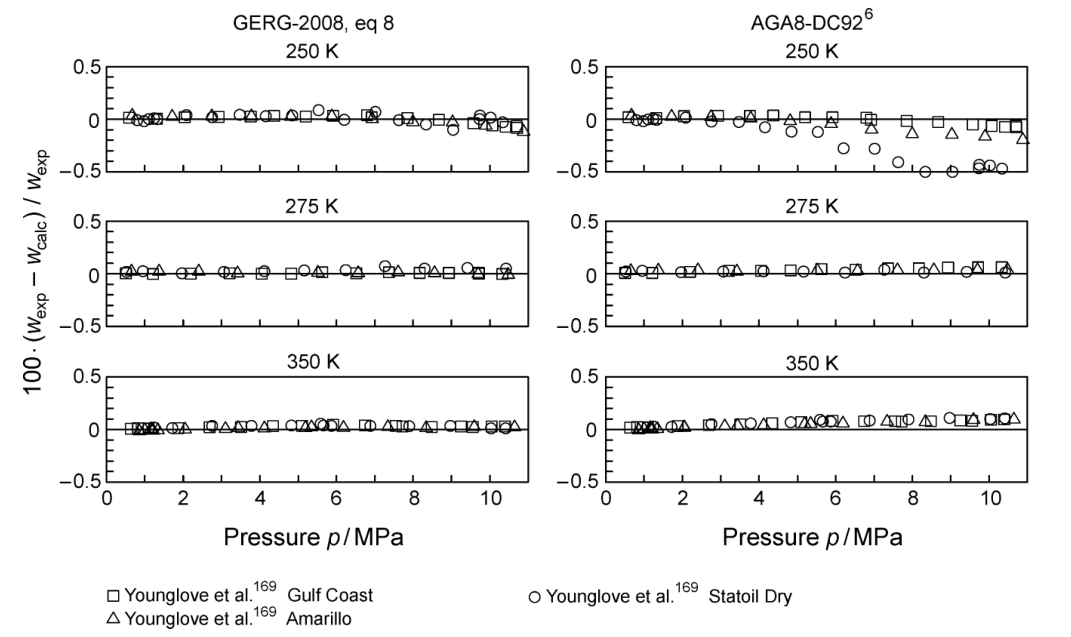
\includegraphics[width=0.8\textwidth]{figs/w2.png} 
	}
\end{frame}

\subsubsection{Punto de rocío}
\begin{frame}
	\frametitle{Punto de rocío}
	Punto de rocío en mezcla de metano, butano, isobutano y pentano.\\
	Y mezcla sintética de $C_1, N_2, CO_2, C_2, C_3, C_4, iC_4, C_5, iC_5,
	C_6, C_7, C_8$ 
	\center{
	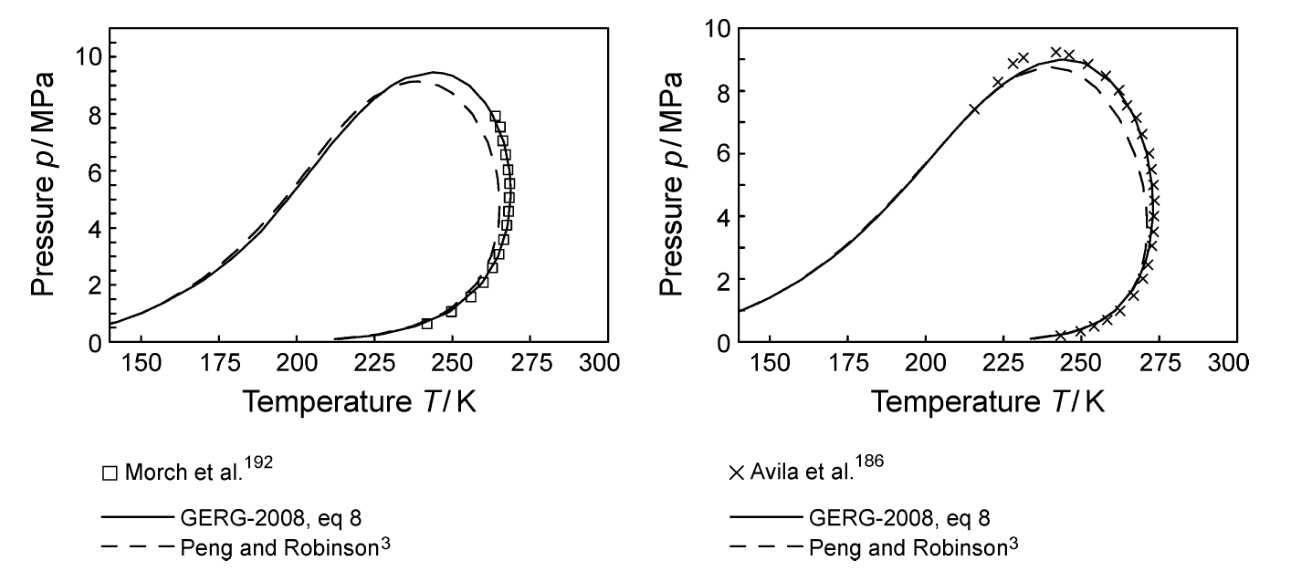
\includegraphics[width=\textwidth]{figs/dew.png} 
	}
\end{frame}

\subsubsection{Punto burbuja}
\begin{frame}
	Punto de burbuja en mezcla Metano-Nitrógeno
	\frametitle{Punto burbuja}
	\center{
	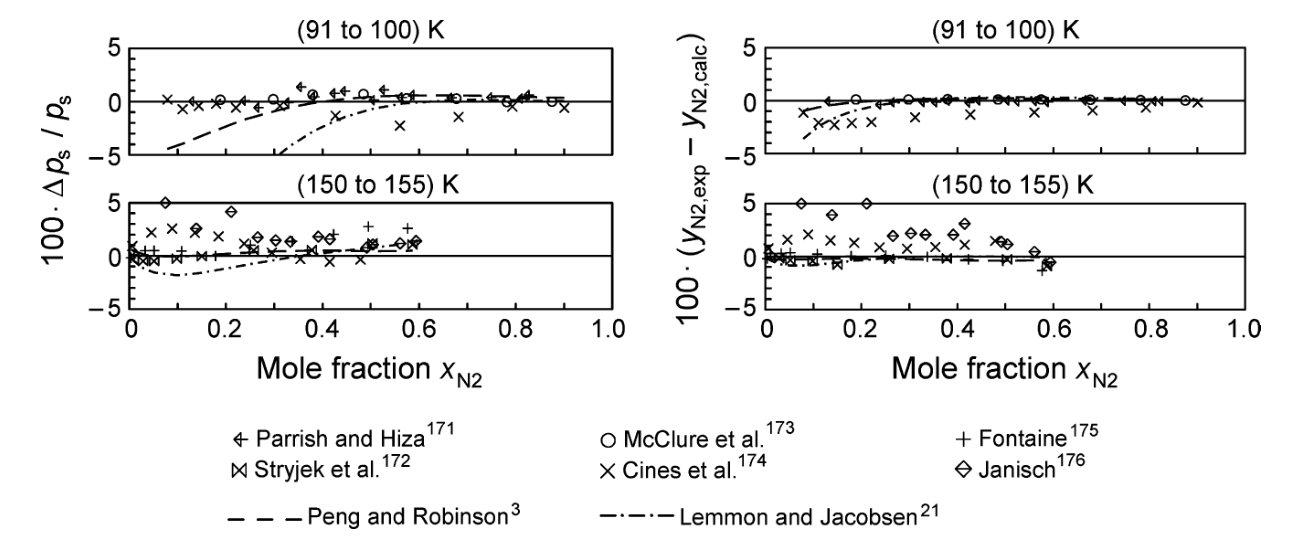
\includegraphics[width=\textwidth]{figs/bubp.png} 
	}
\end{frame}

\section{Conclusiones}

\begin{frame}
	\frametitle{Conclusiones}
	Comparada a otras ecuaciones de estado, la ecuación GERG 2008 logra una
	descripción precisa de propiedades de diversas mezclas sobre rangos de
	temperatura, presión y composición más amplios. \\~\\

	\textbf{Rangos de validez}
	Se dividieron dos secciones:
	\begin{description}
	\item[Rango Normal] Puntos entre:\\
		$90 K \le T \le 450 K$\\
		$p \le 35 MPa$\\ 
		Entre estos rangos las desviaciones se encontraron
		entre 0,1 y 0,5\% para la mayoría de las propiedades.
	\item[Rango Extendido] Puntos entre \\
		$60 K \le T \le 700 K$\\ 
		$p \le 70 MPa$\\
		Al expandir el rango hay ciertas 
		mezclas en donde la incertidumbre de mediciones de 
		densidad alcanza el 1\%. Se considera que puede ser
		utilizada en casos donde mayores incertidumbres sean
		aceptables
	\end{description}
\end{frame}

\begin{frame}[c]
	\frametitle{Referencias}
	\printbibliography
\end{frame}

\titleframe{Muchas gracias!}

\end{document}
